
\section{Getting to know Klimahuset}
\par
\emph{26.01.2021, initial contact and visiting Klimahuset for the first time}
\par

\begin{figure}[H]
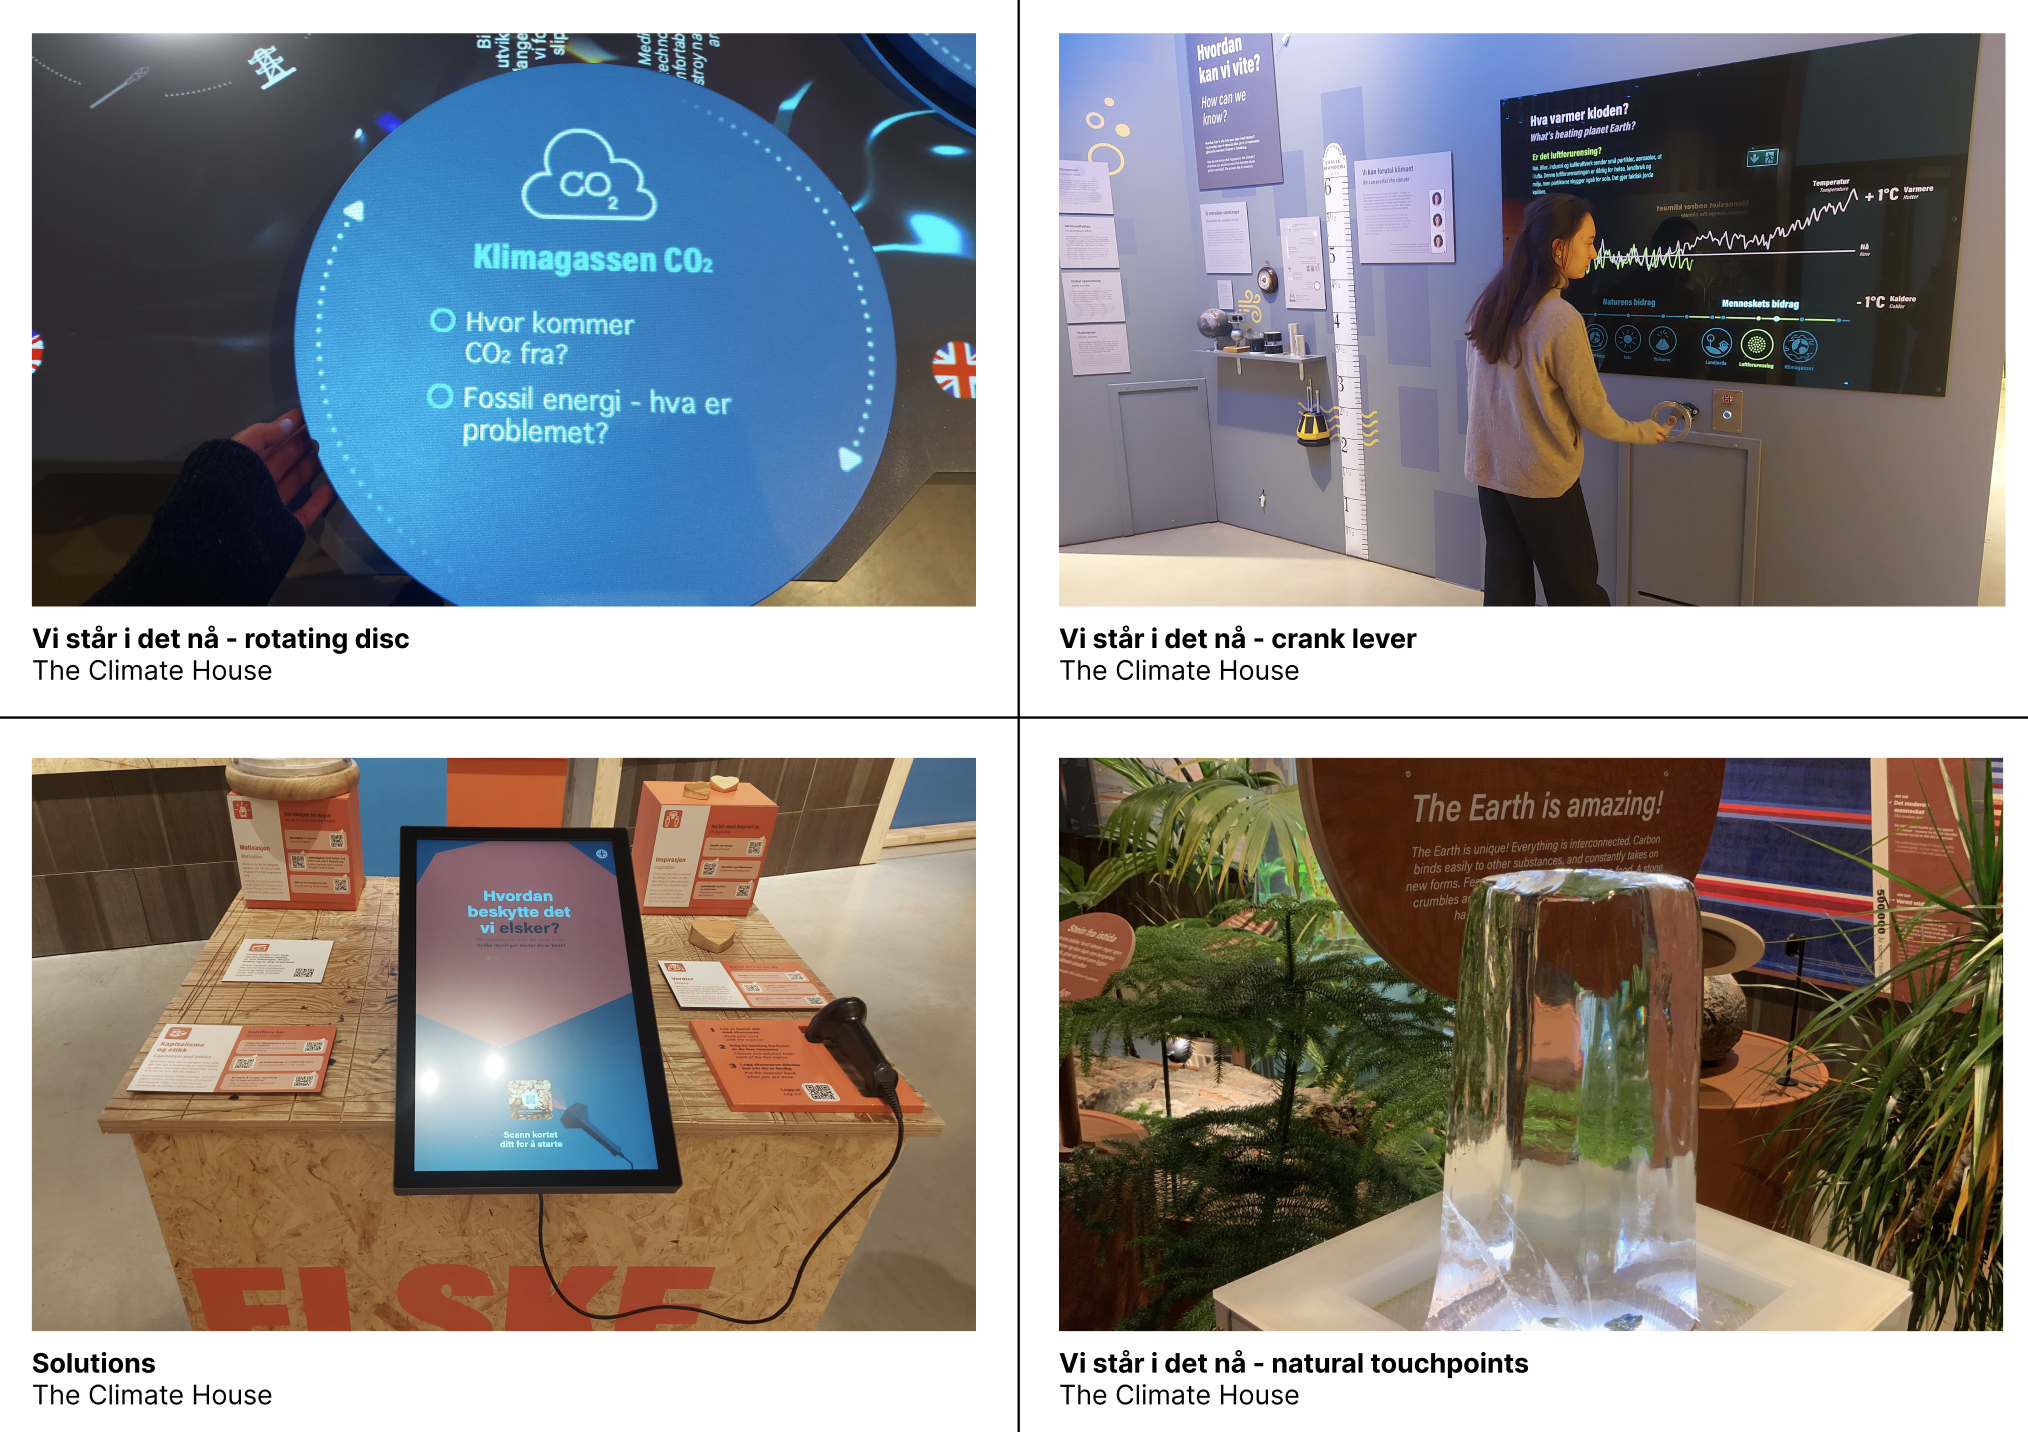
\includegraphics[width=12.5cm]{pictures/klimahuset/klimahuset.JPG}
\caption{Klimahuset}
\centering 
\end{figure}

In the middle of January 2021, covid-19 restrictions started to cease and we were invited to visit Klimahuset and meet our contact person there for the first time. At the time, Klimahuset was a newly opened museum located in Botanisk Hage at Tøyen in Oslo. Because of strict pandemic restrictions from 12.03.2020 and onward, the museum had only been open for visitors a few months prior the official lockdown. This visit in January was our first look at the museum space and exhibition \emph{"Vi står i det nå"}, and we had about 30 minutes to go through the exhibition.

% Should I add a picture with the text "vi står i det nå". ?

In the aftermath of this first meeting, we were given access to internal documents portraying Klimahusets founding museum values, ambitions and vision. The documents went in-depth on the whole process of making the exhibition, starting with Klimahusets founding documents; motivation, requirements and vision for what the museum aimed to address, and who to target. Followed by documentation from the design agency responsible for creating the installations, containing both reasoning and documentation of each installation, as well as the proposed optimal visitor-journey through the space. The first-impression of the exhibition \emph{"Vi står i det nå"} and the founding documents, informed our understanding of what an interactive museum context could encompass. As well what it would mean to design with Klimahuset as the provider of context, not as client.

\begin{figure}[H]
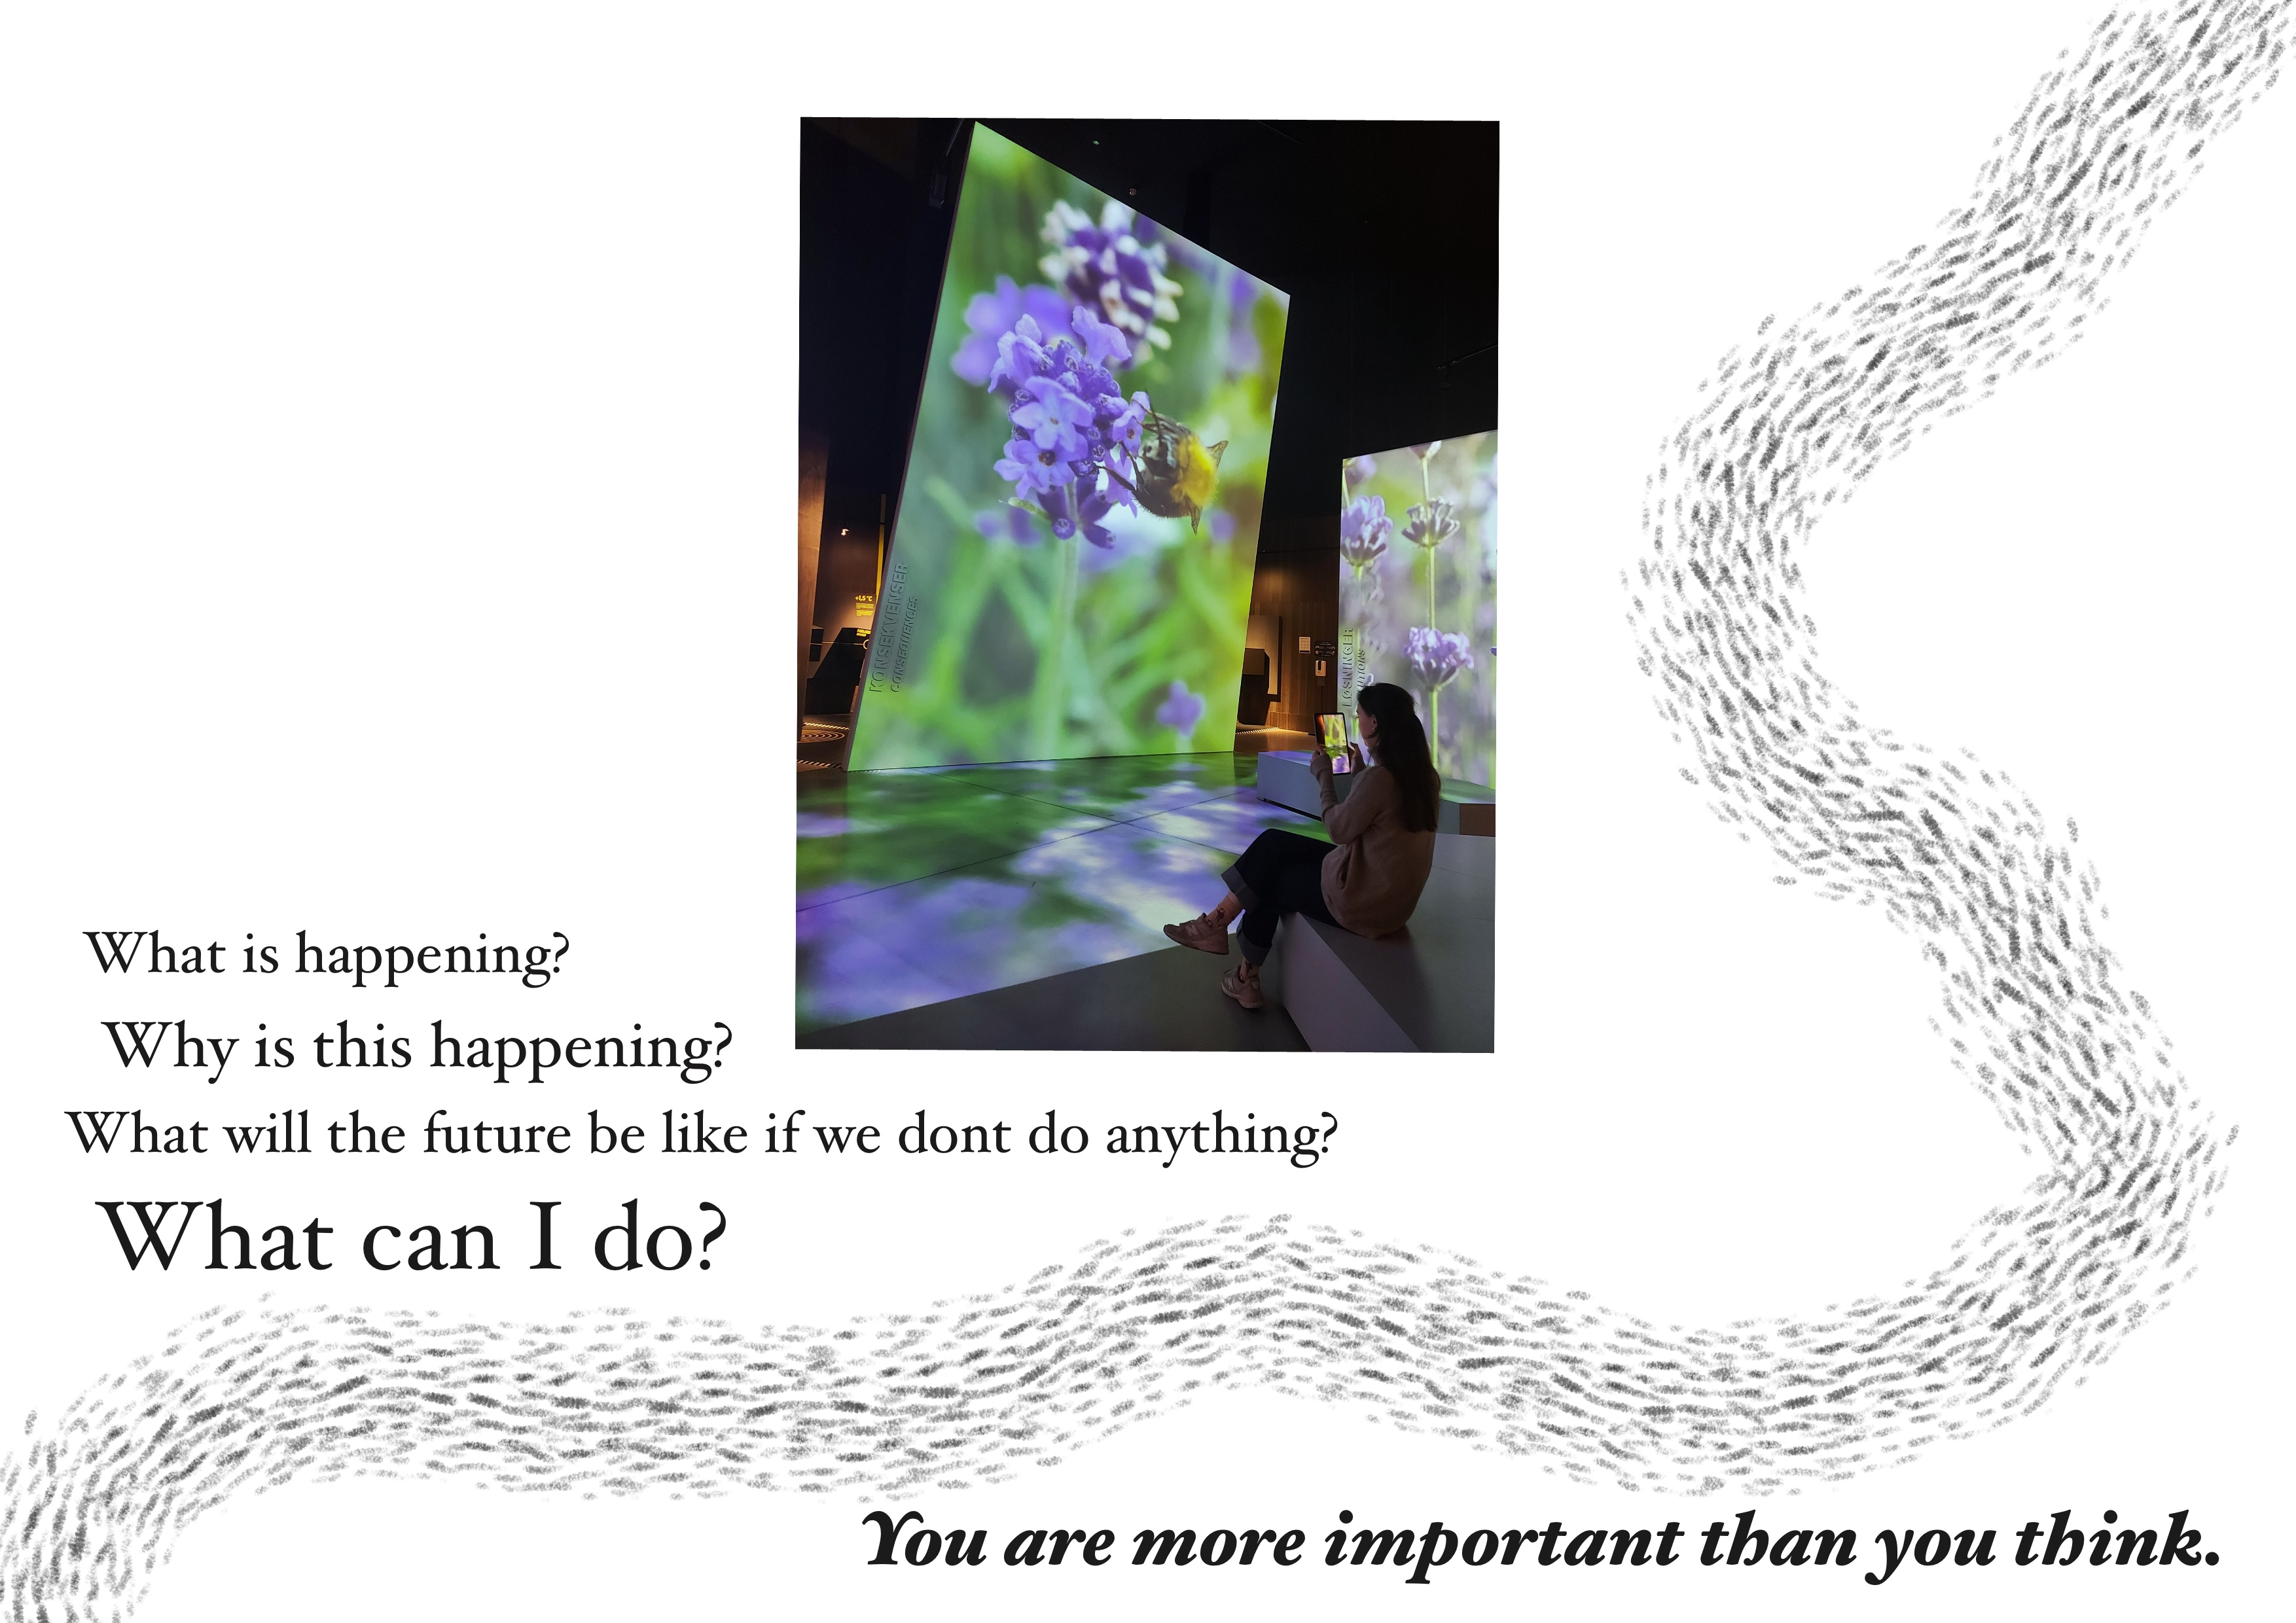
\includegraphics[width=12cm]{pictures/klimahuset/important.jpg}
\caption{Klimahuset want the visitor know that you are an important asset in the fight against climate change, and motivate you to take climate action after the museum visit.}
\centering 
\end{figure}

At this time, the research question I had was quite broad and explorative; \emph{design an interactive visual installation addressing sustainability}. Because the end-goal then was to create an interactive installation that addressed sustainability, I was looking into different topics and values linked to interactivity and sustainability - especially in terms of what the interaction designer's role in the climate debate could be. Walking through a museum is an experience. It should be, and it is curated thereafter; as a journey. Drawing inspiration from service-design thinking, the interaction designers equivalent methodology framework to design an experience involving digital touchpoints or artefacts, I wanted to capture the different elements that made up Klimahusets museum experience. I therefore specifically asked for documentation on Klimahuset's values and visions, architecture- or service blueprints, how they collected feedback from visitors and how they measured engagement. The inquiry was driven by interest in understanding more about how Klimahuset could represent a "modern museum", through studying how they used interactive installations to disseminate, educate, inform and encourage reflections, trains-of-thoughts, conversations or action with its visitors. Through discussions with my peer research buddies, we started questioning which areas in the existing space we wanted to do something similar to, and in general where and how our installation could fit into the existing journey, whilst keeping it’s integrity and independence. How could we complement and bring a new and different perspective into the exhibition journey?

\paragraph{Research inquiries/ interests: }
\begin{itemize}
    \item Wanted to understand more about how a "modern museum" through the use of interactive installations worked to disseminate and engage with its visitors.
    \item Sustainability is a broad term, wanted to specify it to start conceptual work on the installation. To synthesise the design space.
    \item Where and how will the installation fit into the existing journey, and what will it "bring to the table"?
\end{itemize}



% This is where reading on museum context starts 


\section{Investigating narratives and storytelling with Klimahuset}
\par
\emph{08.04.2021, workshop with members of staff from Klimahuset}
\par

In the beginning of April 2021, me and my research buddies were requested to host a workshop for different members of staff from Klimahuset as a way to kickstart the collaboration with the museum. Inspired by readings on narrative theories and learning in contemporary art museums, and the way narratives are constructed in a museum context \autocite{narrative_sitzia}, we saw this as an opportunity to learn more about how narrative play a part in telling a story and in conveying a message. We wanted the workshop to explore how to engage participants in building a narrative, and anticipated that it would give us some insight on how to build climate-crisis related narratives. This would also give us the opportunity to get some input on which sustainability issues can be a better fit, topic-wise, when designing for a learning-oriented type of installation. Lastly, we wanted to facilitate a conversation on the current existing exhibition in Klimahuset, to get some feeling if there were any topics or sustainability issues they wished the current exhibition should address.

We designed the workshop timeline to endure three phases; brainstorming, storyboarding and presentation. Because of the ongoing pandemic we conducted the workshop digitally through Zoom, using Miro as the workshop platform-tool. We primarily wanted to get a better grip on different topics and issues in the climate debate that could be used as groundwork for design fictions, which is why we tried to brainstorm three dimensions that can make up a story; a theme, a dilemma and a setting. Therefore we asked them:

\begin{itemize}
    \item What topics in the climate debate do you think is important to address?
    \item Write down issues/ dilemmas related to climate debates.
    \item Write down (a climate-related) setting.
\end{itemize}

In the next part of the workshop we wanted the participants to create their own individual storyboard, where they could choose between all commonly brainstormed themes, dilemmas and settings - to make up their own story that they would later present. And then to finalise the workshop, the participants presented their own story. It was interesting to see the diversity and different perspectives from the participants and their respective stories. Even though some participants had used the same theme, dilemma or setting, they all differed in terms of what the participant wanted to convey with their story. 

In the aftermath of this workshop, the collected stories and notes from the discussions have worked as a foundation for me to look into the relationship between narratives, dissemination in museums and meaning-making. The main finding I got from the workshop is the notion on how a well written narrative have the power to make us think about or see ourselves and the Earth around us with new eyes, enabling us to engage in and relate to the climate crisis through the narrative that is told. The climate crisis is first and foremost a story about humans and humanity, and the power in the narrative therefore lies in the message conveyed. 

\begin{figure}[H]
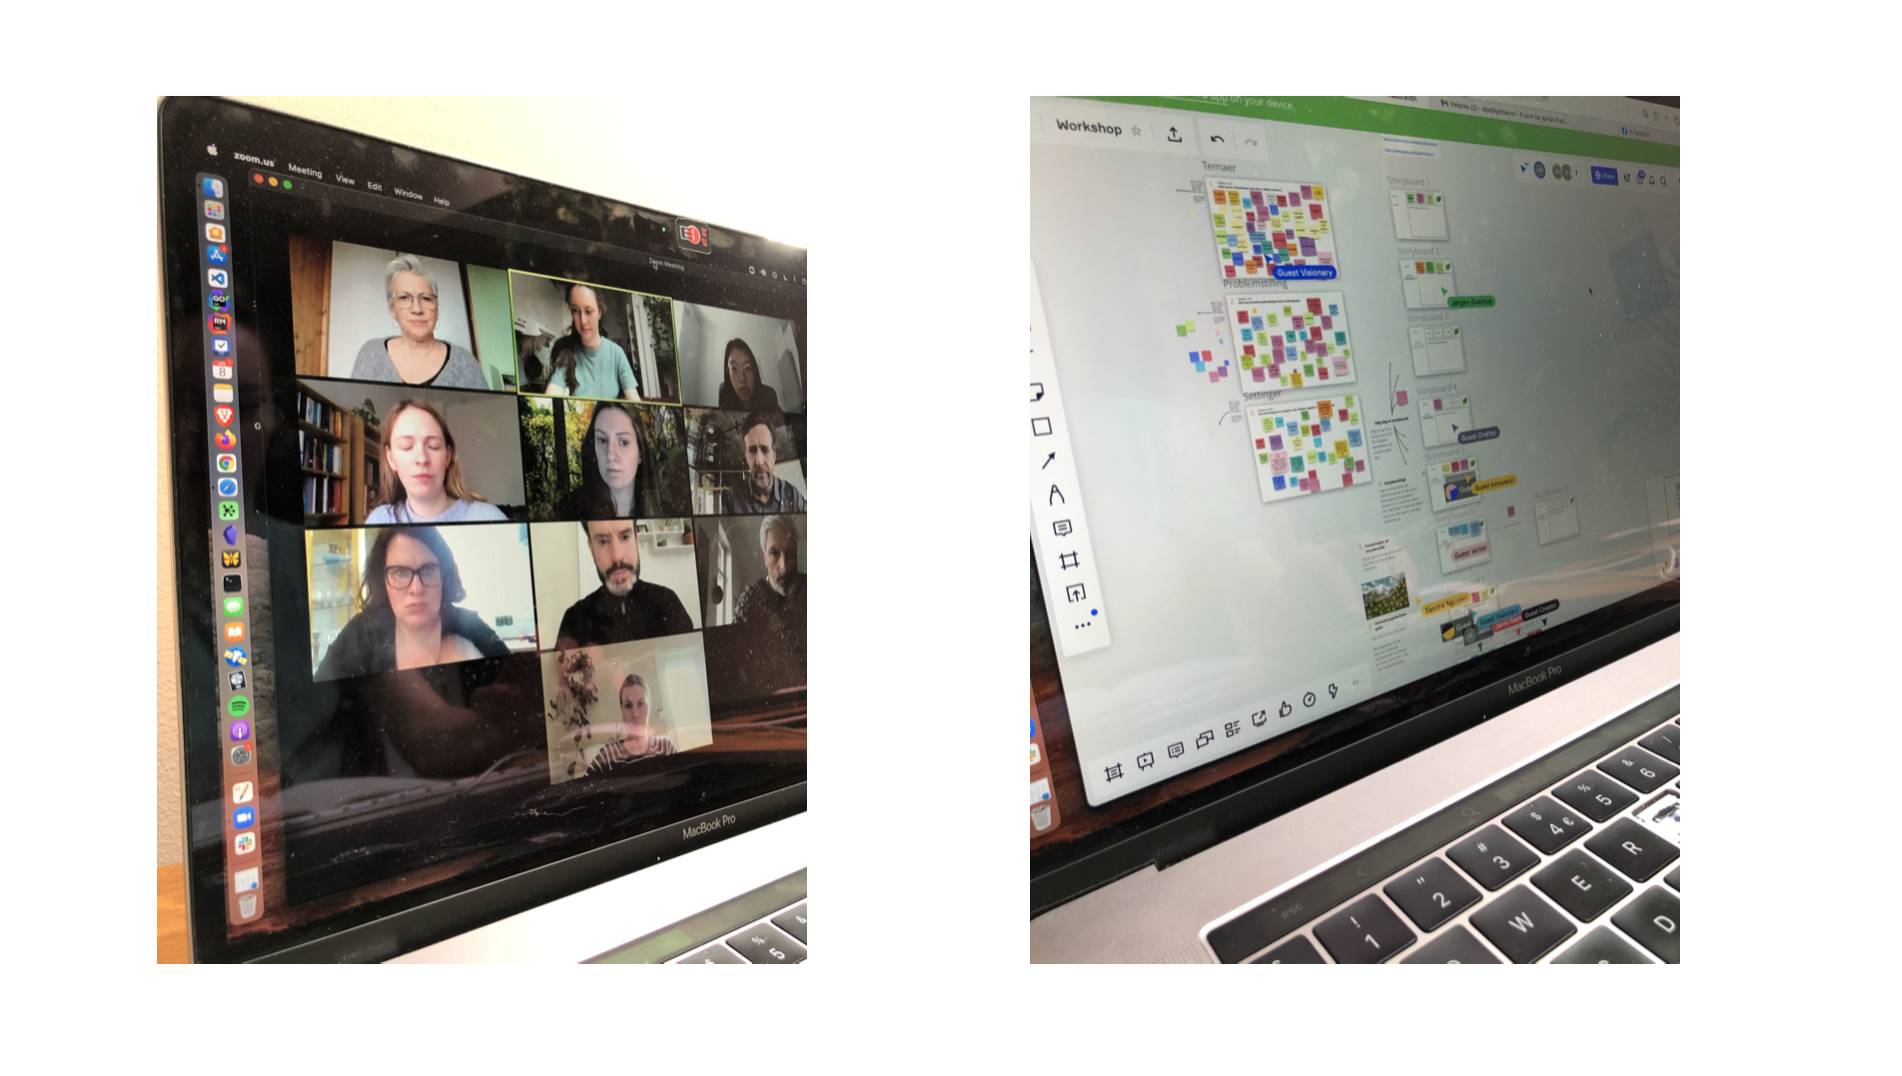
\includegraphics[width=13cm]{pictures/narrative_workshop.png}
\centering 
\end{figure}


TODO: Add workshop guide in appendix, and elaborate more on the actual workshop design. Account for the choice behind the workshop design, and be more clear about what the RQ and research motivation at the time was. And also what lessons learned I/we had, and how that affected the way forward.

After the workshop we started conceptualising new ideas and concepts. Inspired from the workshop, but also research.

\begin{figure}[H]
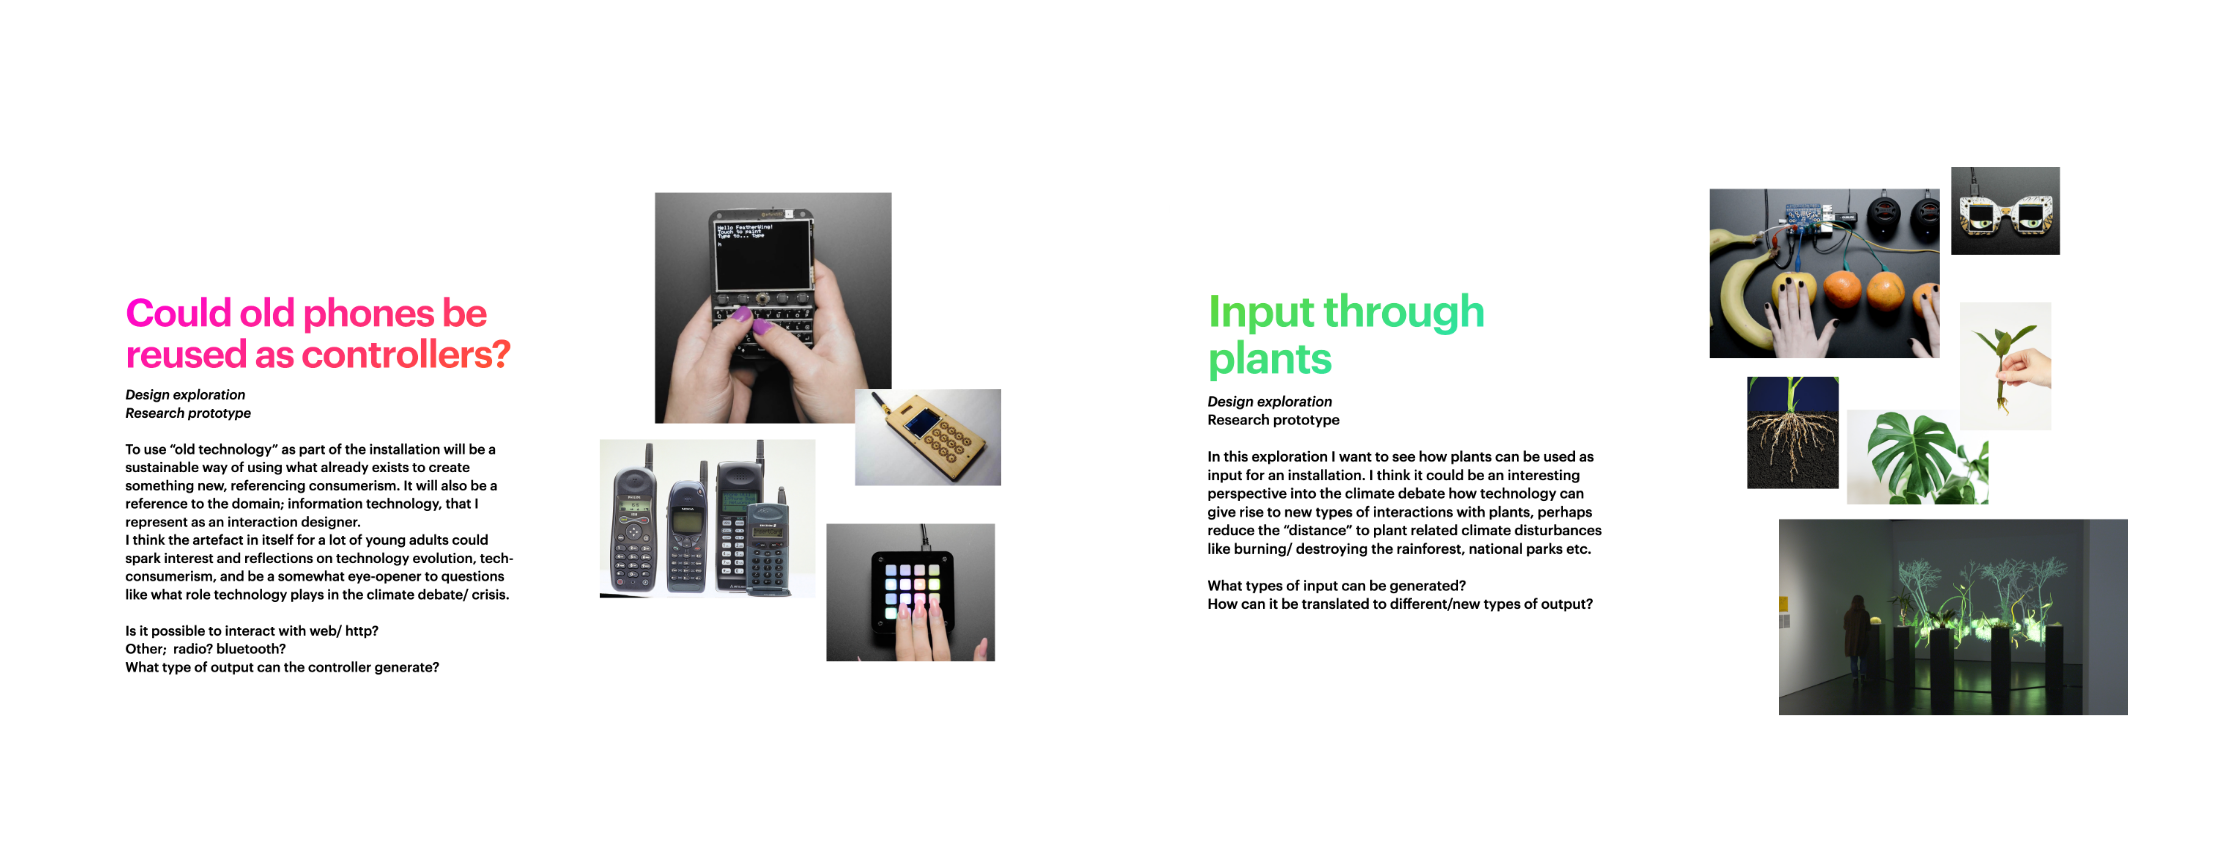
\includegraphics[width=13cm]{pictures/process/mini_pitches.png}
\centering 
\end{figure}

\section{Exploring input through plants}
\par
\emph{01.05.2021, presentation at Klimahuset}
\par

The thought behind this project was to explore how human touch on plants could be used as input, or as a type of controller, to manipulate elements of the installation. The statement of using an actual, living plant would be a direct reference to the relationship between human and nature: plants, animals and ecosystems, bringing nature closer to the discourse where sustainability issues are discussed, inviting to reflections to the ecological damage that we are responsible for. I think this exploration addresses the research question as to how interactive artefacts can provide new depth to the museum discourse, by exploring how human touch through plants can stimulate emotions or values like empathy and awareness, reinforced by the educational environment (the whole museum) the installation is placed in. I believe the plant installation could be interesting to use in combination with learning about plant/ nature related climate disturbances like the burning and destroying of the rainforest, but also in a local, Norwegian context; the windmill debate, hydropower, national park borders, repercussions of cottage development or light pollution. During the shaping of this exploration, I managed to define yet a research question that I want to inquire into; can new/different interactions with natural objects contribute to increased climate consciousness and activism?	

\begin{figure}[H]
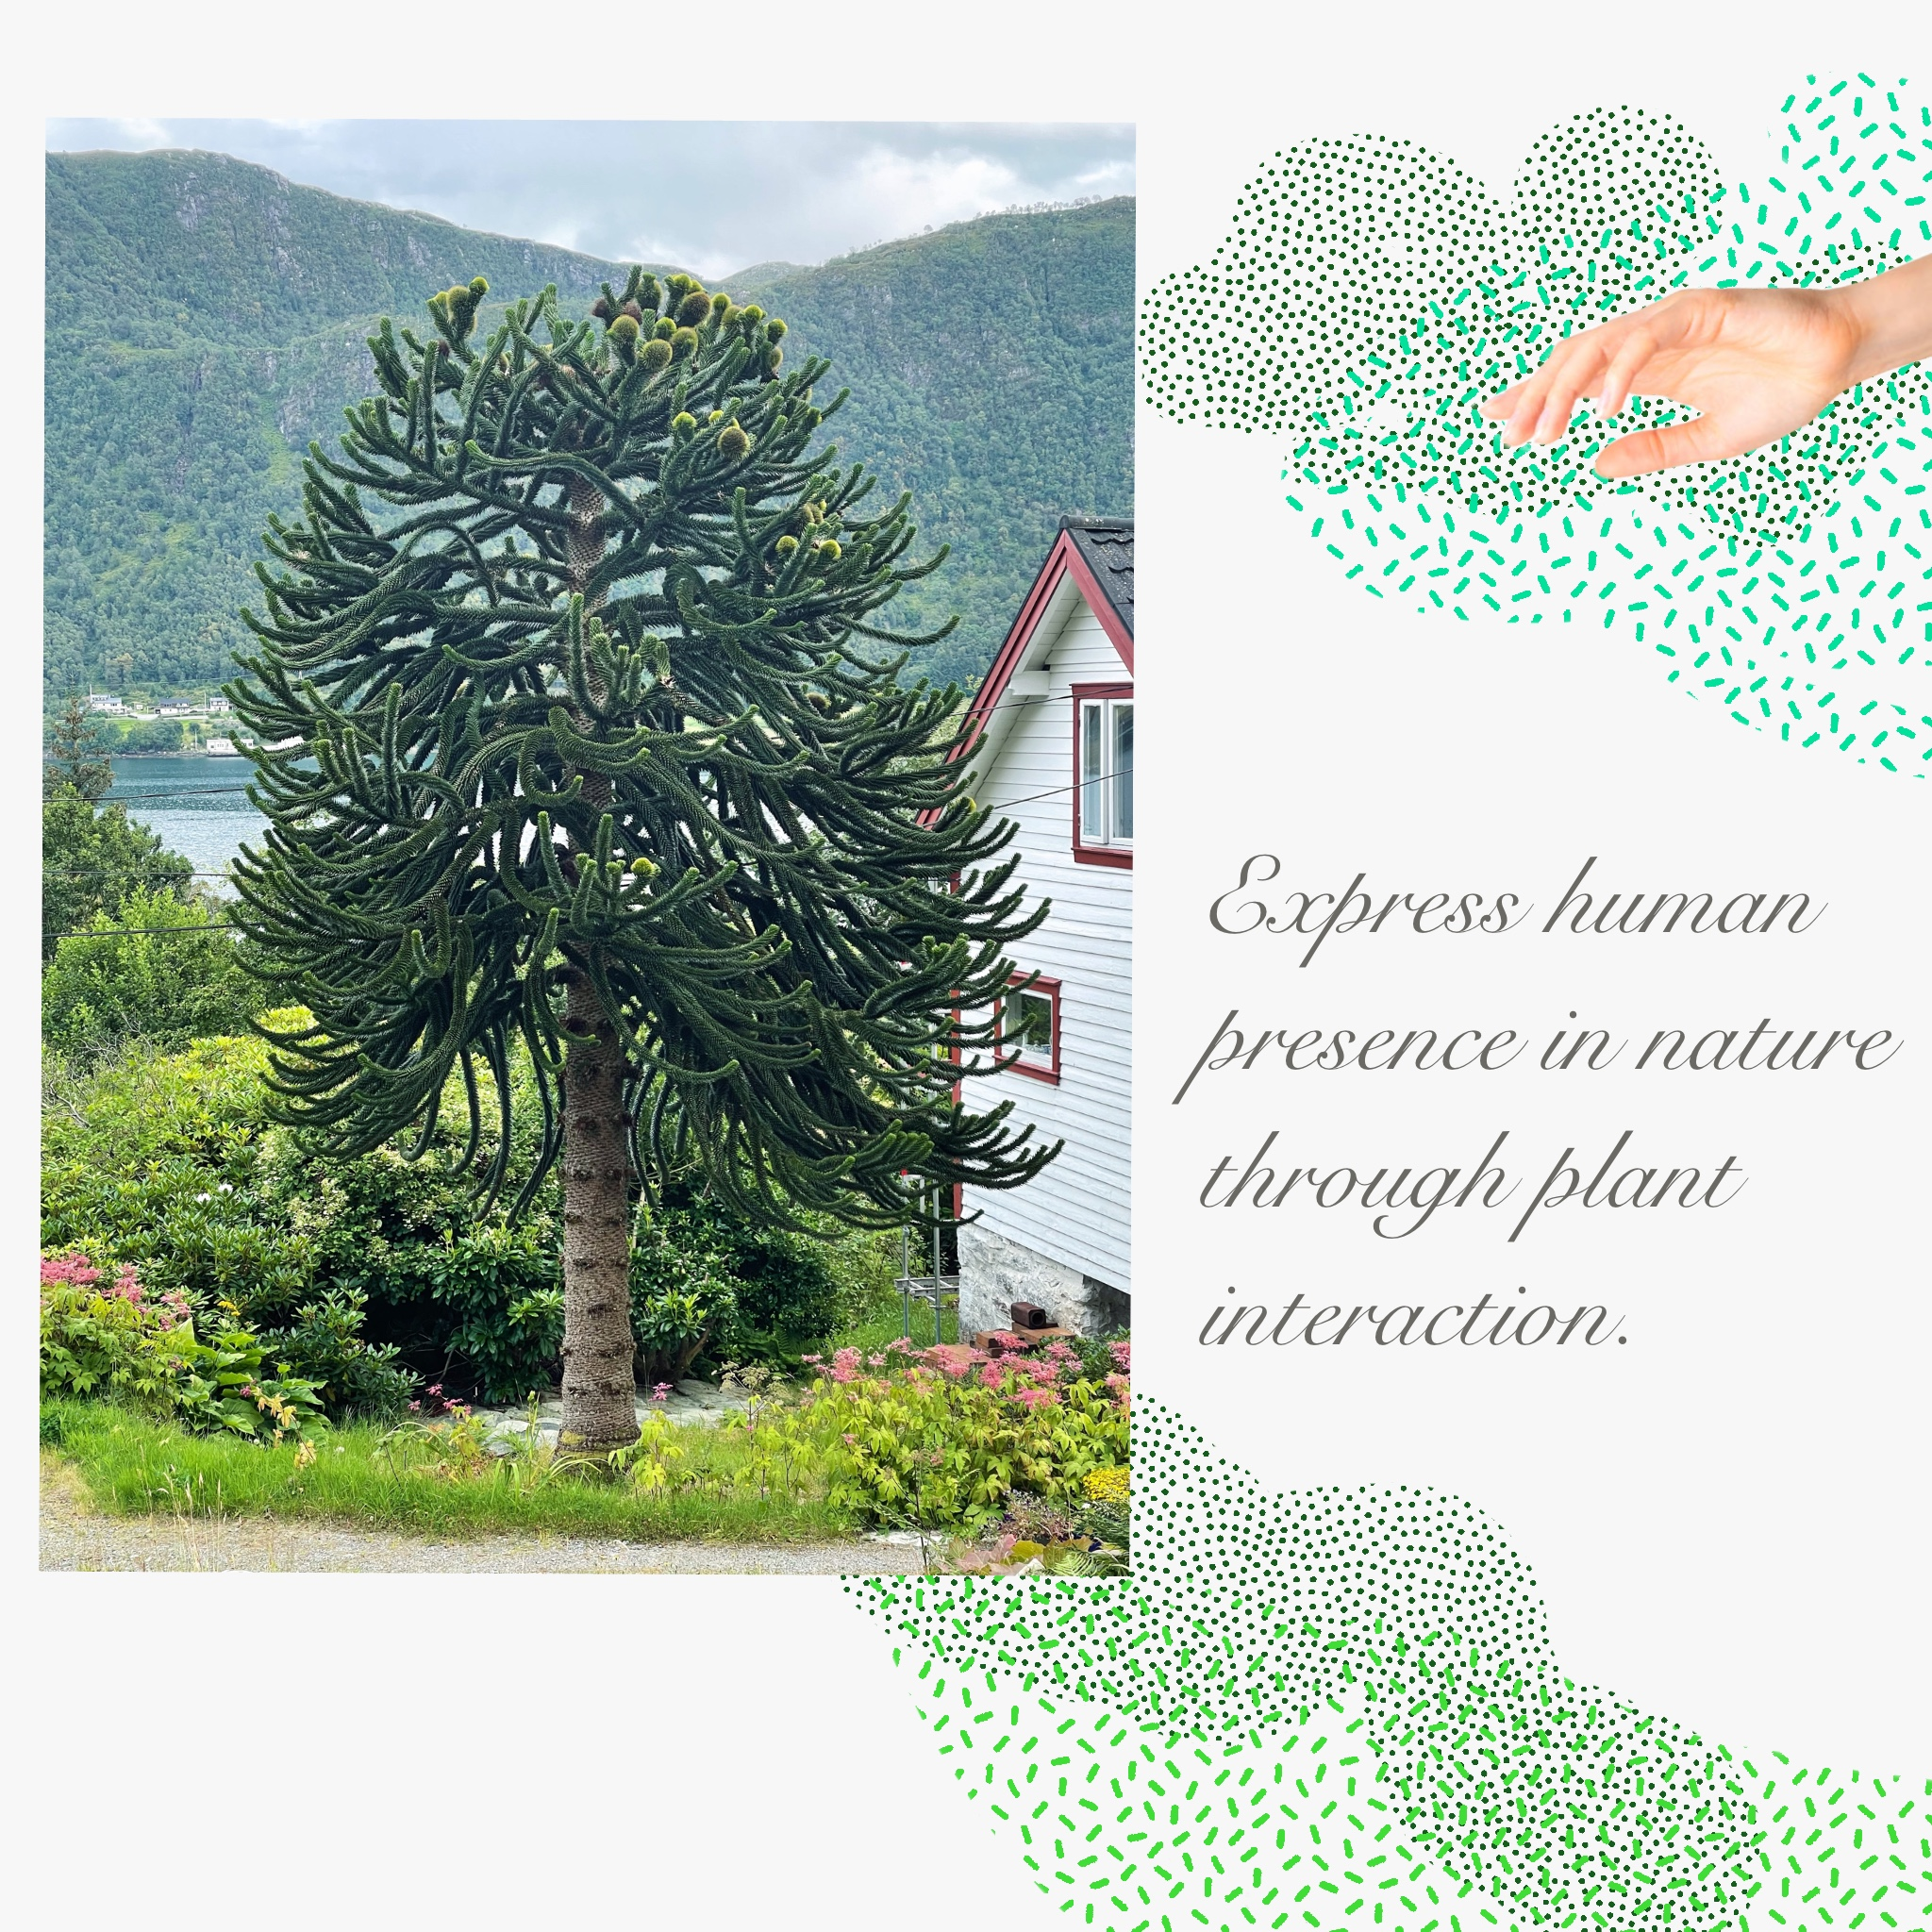
\includegraphics[width=13cm]{pictures/human_presence.jpg}
\centering 
\end{figure}


\section{Slow Design: Qi}
\par
\emph{25.08.2021-01.10.2021, tangible interaction intensive course}
\par

In September 2021 I took part in an intensive studio course called Tangible Interaction (IN5470). Each year, a theme is given that the students explore in a project that spans most of the five weeks this intensive course lasts. This year's theme was Slow Design, and in groups of three we were challenged to design and create a fully operational installation by the end of the course, and unveil the installation in a joint exhibition along with the other groups. We were 


\subsection{Memento Mori}

\begin{figure}[H]
\includegraphics[width=10cm]{pictures/process/memento_mori.pdf}
\caption{}
\centering 
\end{figure}

\subsection{Presence in Existence}

\begin{figure}[H]
\includegraphics[width=10cm]{pictures/process/presence_in_existence.pdf}
\caption{}
\centering 
\end{figure}

\subsection{Qi}

\begin{figure}[H]
\includegraphics[width=10cm]{pictures/process/qi.pdf}
\caption{}
\centering 
\end{figure}


\section{I/O (In Oslo) by Yuko Mohri}
\par
\emph{22.10.2021, excursion to Atelier Nord}
\par

In late October, me and my research buddies visited Atelier Nord to see and analyse the ongoing exhibition by Yuko Mohri: I/O (In Oslo). Going in, we expected the exhibition to be or have interactive qualities, and my research interest during this fieldwork was guided by \autocite{hybridplace_ciolfi}'s Hybrid Place dimensions. 

This is how Atelier Nord describes the installation: 
\emph{Gently cascading rolls of paper are fixed to a framed structure in the ceiling and pick up dust and other debris. The traces are scanned and converted into random input-output signals that case a constellation of objects, such as feather dusters and old musical instruments, to move and produce sound. The site-specific characteristics - including movements of air, humidity, and the undulating surface of the floor - are picked up by the rolls of paper, gradually permeating it with the unique features of the exhibition space. The result is an organic environment where the same sound and movement never occurs twice. In this case, the gallery might be likened to a biotope-like ecosystem that interweaves the natural and artificial.} \autocite{yukomohri_web}

What follows is an experience account?
Guided by the Hybrid Place framework, I first looked for the physical and structural qualities of the space. I noted how the showroom was large, kind of empty and very open. The installation itself consisted of two separate installations, both placed in the center of the room, so that visitors could walk both around and in-between the two installations. There was also a small room where the visitor could see a movie about Yuko Mohri and her thoughts behind the installation. There was no tape on the floor, or signs saying to not touch or walk, and in that sense the showroom invited to make our own path and discover the installation in our own pace and way we wanted. The showroom was pretty small, perhaps around 30kvm, and aesthetically quite plain. The wooden floor creaked when walking, and the sound echoed through the space. There was no music or what-so-ever in the background, only faint city-noises from one side of the housing and rustling of leaves from the other. The installation produced sound randomly from two outputs; feather dusters and an old musical instrument. During our visit we only heard the thumping from the feather dusters you can see depicted above. I noted how "clacking" sounds from both my own and other visitors shoes directed the attention toward movement in the room. The effect were especially reinforced after standing still for a while, looking, thinking about the installation. I noted that in the moment, sound and movement produced by the other visitors in the room influenced my mental presence being drawn back-and-forth, in-and-out, from the mind-space I was present in when observing and thinking about the installation, and then drawn back again to the physical space. Because of the showrooms atmosphere as I just described, and the room being small, it's easier to meet eye-to-eye with the other visitors, listen in on their conversations, and simply being aware of their presence. It felt a little awkward to talk, and sometimes also to move, resulting in a quiet/ whispering way of communicating with my research buddies during the visit.

\begin{figure}[h]
    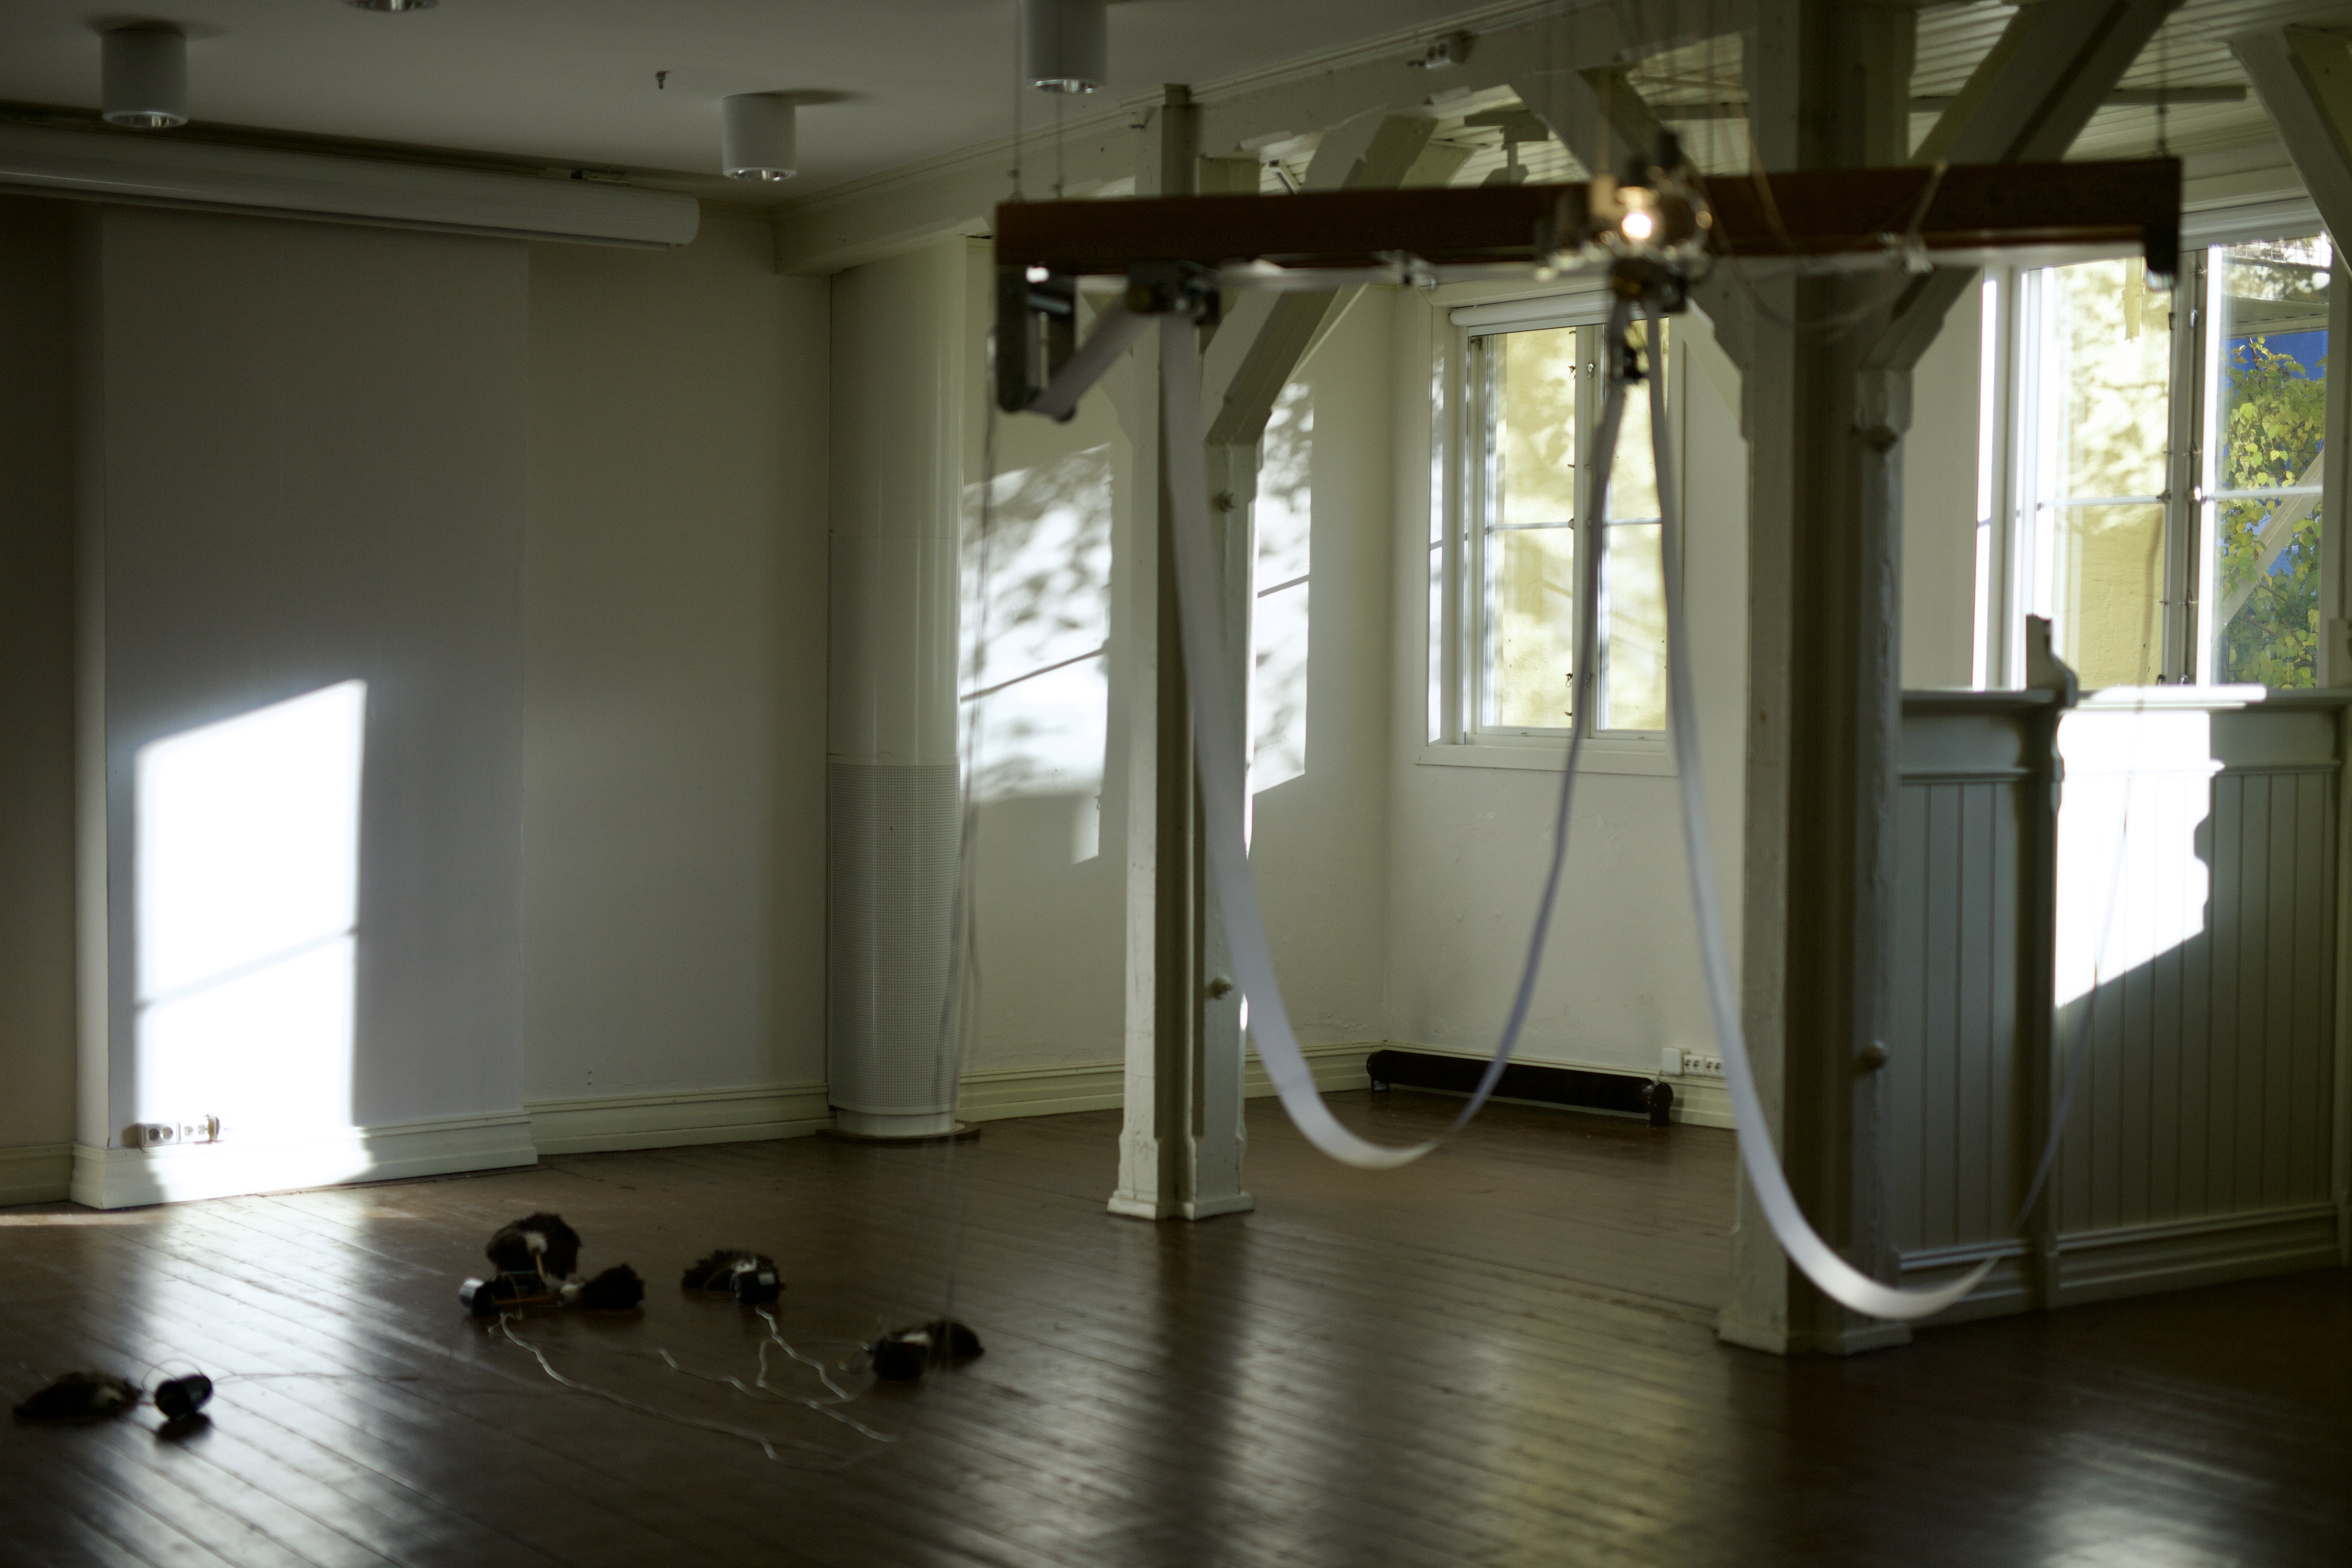
\includegraphics[width=12cm]{pictures/process/yuko_harmony.jpeg}
    \centering 
    \caption{Notice how the sunlight add a layered meaning to traces in the air being picked up by the cascading rolls of paper.}
\end{figure}

In terms of the physical/ structural dimension \autocite{hybridplace_ciolfi}, I would say that the space support group interactions, but it doesn't favour it. Therefore, I noted that the exhibition did not fit into the social dimension of the Hybrid Place framework. Coming into the showroom in a group of three, we actually had the space to ourselves for quite some time, but we walked around in silence for most of that time. Eventually, two people entered, and we were then not alone. Because we already had been there a while, we shifted focus from the details in the installation and how it worked, to see how the pair moved around and used the space. The presence of a new group of people did not change the atmosphere as I described, they were also walking slowly, talking in a quiet manner and payed attention to the way we moved around the installation as well. Perhaps they assimilated us, or the atmosphere we created? I actually did not notice the video-room before these two new people entered, as this was the first thing they did after talking to the Docent and orienting themselves in the space.

When it comes to the last two dimensions, the cultural and personal dimension \autocite{hybridplace_ciolfi}, I have only categorized the 

+ personal
+ cultural


\begin{figure}[H]
\includegraphics[width=12cm]{pictures/process/yuko_presence.jpeg}
\centering 
\end{figure}

The Docent who was in charge of the space and exhibition was quiet, looked tired, and did not initiate any dialogue or conversation about the installation. We were kind of just left to ourselves the entire time.


\begin{figure}[H]
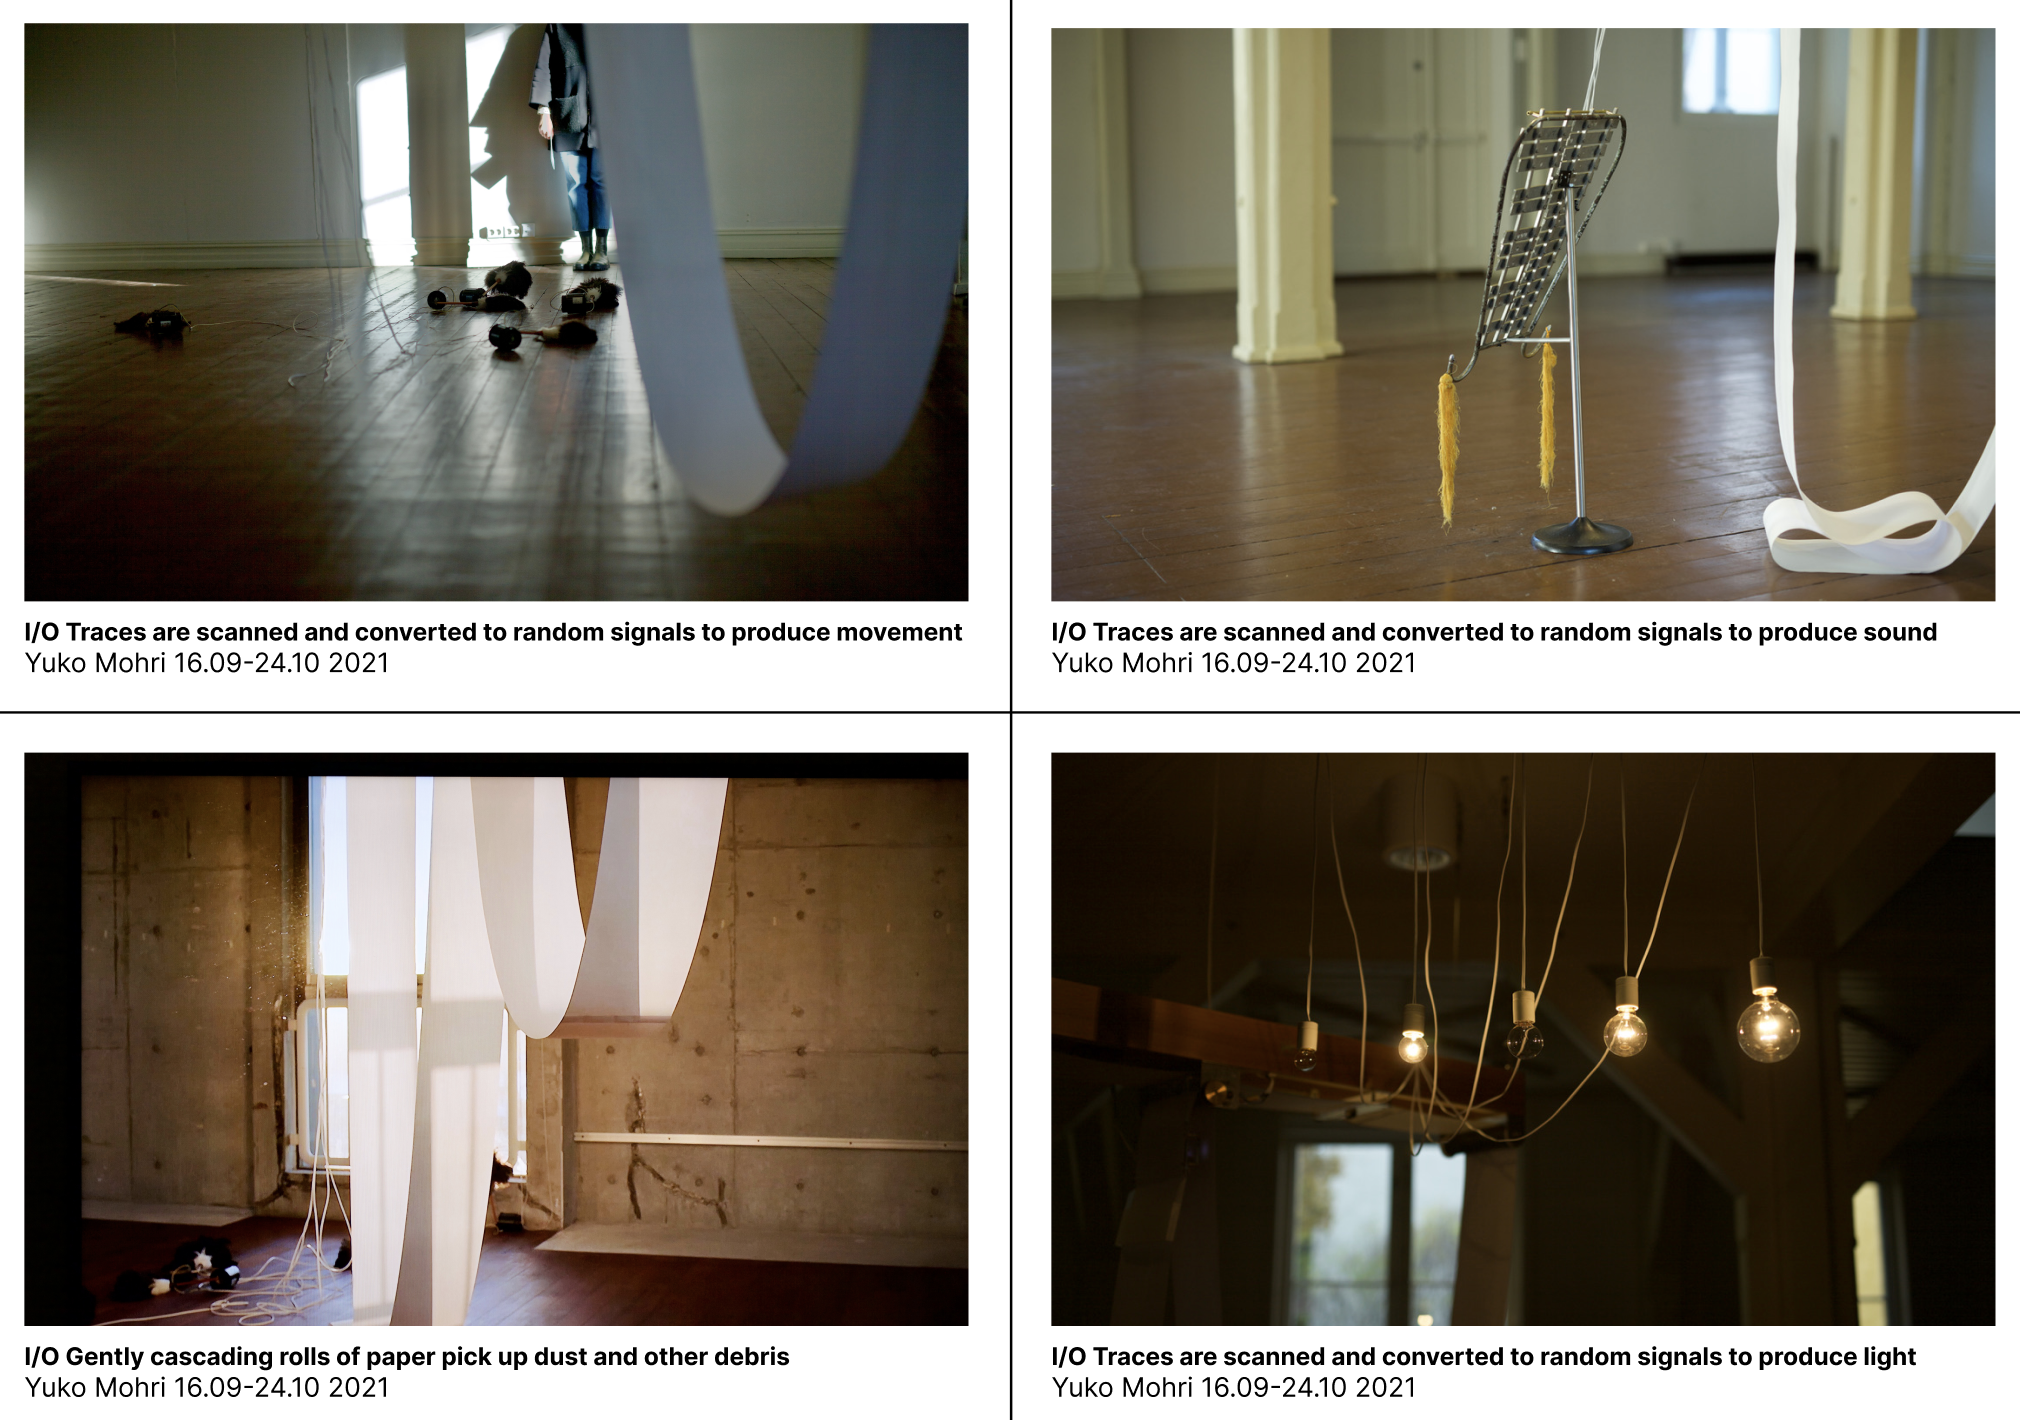
\includegraphics[width=12cm]{pictures/dataset/yuko_mohri.png}
\centering 
\end{figure}


\section{Poison by Munch}
\par
\emph{27.10.2021, excursion to Munch Museum w/ focus on the temporary exhibition Poison}
\par

A couple of days after we visited 
Munch is a great example of how they use text and plaques to inform/guide the visitor in terms of how they can read some of the art they see. It is a good example of how one can design the visitor journey through the exhibition space. It supports the visitors sense-making, in terms of how they can use and move through the space. However, it is an analogous way to support sense-making, while I am interested in ways interactivity can support this type of sense-making. Even in the interactive Poison exhibition, the information is static.

\begin{figure}[H]
\includegraphics[width=12cm]{pictures/process/pink_munch.jpeg}
\centering 
\end{figure}

\section{Shadows by Munch}

\section{Kistefoss museum}

\section{Qi: Energy visualisation workshop}
\emph{09.11.2021, invited to host an energy-visualisation workshop}
\begin{figure}[H]
\includegraphics[width=11cm]{pictures/dataset/Qi.pdf}
\centering 
\end{figure}

\section{Haptic Interaction}

\section{Observing Klimahusets narrative storytelling in-action}
\par
\emph{Observation and interview 16.02.2022}
\par

After my readings on the museum and its expository agency, I wonder what Klimahuset’s stakeholders thoughts are on their agency? And their position toward whether or not they have a subjective or objective expository agency? What are the cultural attitudes, decisions, views and stances the agents involved in designing the climate exhibition in Klimahuset, took before they decided to do the act of exposing? What cultural function does the objects on display in Klimahuset pose? 

Some of these questions can already kind of be elaborated for, from initial reading on internal documents that I have gotten access through collaborating partners in Klimahuset, as well as from conversations with stakeholders from Klimahuset last semester through the workshop, mail correspondence and mini-exhibition. As accounted for in Klimahusets founding documents, their vision/ purpose of the museum is as follows:
To give the visitors an understanding of the most important climate processes that affect the living conditions on Earth so that they are able to develop their own views on climate change, take part in climate discussions or act in other ways in relation to the topic.
Visitors must gain an understanding that natural conditions also affect social structures and culture.
	
Building on Mieke Bal’s narrative analysis on cultural imperialism in museums, say we look at Klimahuset as an ethnographic museum with the expository agency to display installations, objects and data related to the climate crisis. And with a distinct and clear target group being children aged 10-14. Is Klimahusets agency and vision an attempt to display the climate crisis as a current/ ongoing discourse with the function to educate and stimulate critical reflections on current societal norms and ways of living, or is the agency to define and lay up cultural change, to a more sustainable way of living? Maybe both? If so, then comes the question if the museums cultural stakeholders, with this expository agency, are they cultural moralists? Especially because their whole museum exhibition are designed to engage children aged 10-14, though welcoming all age groups, raises the question if the museum and exhibition design in itself potentially have any moral imperialistic function as well, as to who the discourse (the climate crisis) is relevant for. 
Asked the klimaverter about  this, need to do some structural analysis of some sort….

\begin{figure}[H]
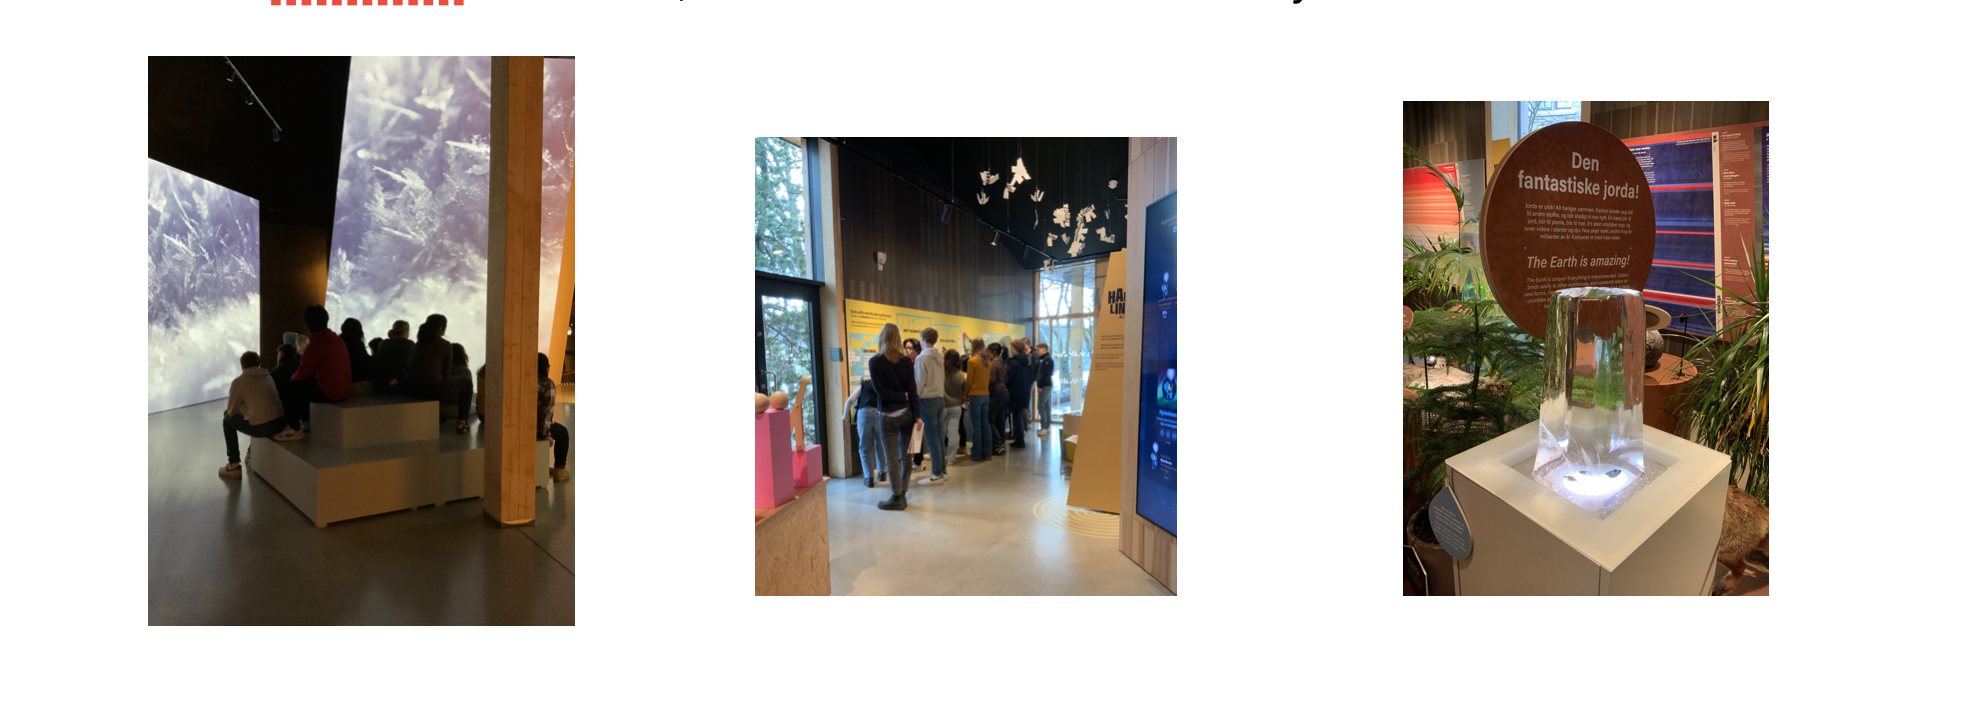
\includegraphics[width=13cm]{pictures/elever_i_klimahuset.png}
\centering 
\end{figure}

Med en klimavert til stede får man bedre hjelp og en form for retning til å “lese” installasjonene, som støtter deg når du senere går gjennom avdeling for avdeling. 
Man blir stilt spørsmål som er knyttet til faktiske ting, som for eksempel i video-atriet sier klimavert; jeg er 160cm høy, hvor høy tror dere denne veggen er?
Etter litt håndsopprekning får vi vite at dersom Grønlandsisen smelter vil havet stige like høyt som det den veggen er. Det er tankevekkende og setter inntrykk!

Her blir man også litt senere spurt: ser dere vær eller klima? et åpent spørsmål som setter i gang en god diskusjon på forskjellen mellom vær og klima, med fokus på hvordan vær påvirker klima. Dette blir forklart at mange blander og tenker at vær og klima er det samme, og at klimaforandringer og værforandringer ikke er det samme. Her får noen elever aha-øyeblikk.


Et annet eksempel er isbiten inne i “den naturlige avdelingen”.  Først får elevene i oppgave å finne noe i området som påvirker klimaet naturlig. Senere når det blir tatt en liten runde spør verten; har alle tatt på isbiten? For så å gå videre til å forklare hvordan menneskelig påvirkning påvirker klimaet. “For eksempel har deres varme hender bidratt til å smelte litt av isbiten her i Klimahuset”. Dette er også tankevekkende og setter inntrykk!


Ice Cube: a good example of a meaningful exp. !!!


\section{Interview with a concept developer from Munch}
\par
\emph{date date date}
\par


